\documentclass[comsoc,final]{IEEEtran}
\usepackage[utf8]{inputenc}
\usepackage[T1]{fontenc}
\usepackage[zerostyle=b]{newtxtt}
\usepackage{subcaption}
\usepackage[inline]{enumitem}
\usepackage{graphicx}
\graphicspath{{figs/}}

\IEEEoverridecommandlockouts

\usepackage{amsmath,amssymb,amsfonts}
\usepackage{algorithmic}
\usepackage{textcomp}
\usepackage{xcolor}
\usepackage{lipsum}
\usepackage[english]{babel}
\usepackage{csquotes}

\newcommand{\todo}[1]{\textcolor{red}{#1}}

\usepackage{hyperref}
\hypersetup{
    colorlinks=true,
    linkcolor=blue,
    filecolor=magenta,      
    urlcolor=teal,
    pdftitle={Iscc2023 Paper}
}
\usepackage{xurl}


\usepackage[style=ieee,doi=false,url=true]{biblatex}
\AtEveryBibitem{%
  \clearfield{note}%
}
\addbibresource{tebaka2023.bib}

\begin{document}    % 6 Pagine, Double Column

\title{\textsc{TEBAKA}: Territorial Basic Knowledge Acquisition. An Agritech Project for the Italy}
%\thanks{Tebaka thanks}
\author{\IEEEauthorblockN{Lorenzo Epifani, Antonio Caruso}\\
\IEEEauthorblockA{\textit{Dept. of Mathematics and Physics "Ennio de Giorgi", University of Salento, Lecce, Italy}}}

\maketitle

\begin{abstract}
Tebaka, proposal, impact, some work. \lipsum[1]
\end{abstract}

\begin{IEEEkeywords}
digital agriculture, precision agriculture, satellite images, deep learning, machine learning,
sensor networks and iot
\end{IEEEkeywords}


\section{Introduction}
% general intro to agritech and relevance for computer science.

The enabling technologies of distributed sensor networks, internet of things, remote sensing using multi-spectral cameras on satellites, drones and aerial platforms, together with smart decision support systems are key contributors for the emerging field of \emph{Digital Agriculture} (DA) or \emph{Agriculture 4.0} \cite{de2018agriculture}. 
This is an \emph{umbrella term} used to designate the transformation of farming that includes digitalization and automation of farming tasks. This area of research encompass a new vision of the farming industry as a cyber-physical farm, and includes all technological areas such as: big-data platforms, machine learning and data-driven models to relate the observations of the phenological stages of plants with field yield and crop quality. 

The high-level goal is to support agronomist with \emph{Precision Agriculture} management practices, to better solve the challenges and demand of an increasing world-population, rising production costs (like energy), labor shortages, climate and environmental changes (like water resource scarcity). It leverage extensive knowledge acquisition using remote sensing technologies, and on-the-field deployment of sensors and IoT networks, to improve knowledge acquisition and situated situation awareness, to maximize resource usage and crop yield while minimizing associated costs.

In the United States, the use of yield-maps and soil maps are adopted only by 5 to 25 percent of total U.S. farms; on the other hand, automated guidance, has increased sharply, with the advance in deep-learning applied to computer vision, and it is applied to over 50 percent of the cultivated areas. A good survey of the trend in the technology evolution of a \emph{Smart Farm} in USA is in \cite{mcfadden2023precision}. USDA (The U.S. Department of Agriculture) is investing up to $2.8$ billion in $70$ selected projects under the first Partnerships for Climate-Smart Commodities funding pool, as a part of the Inflaction Reduction Act.


\begin{figure}
    \centering
    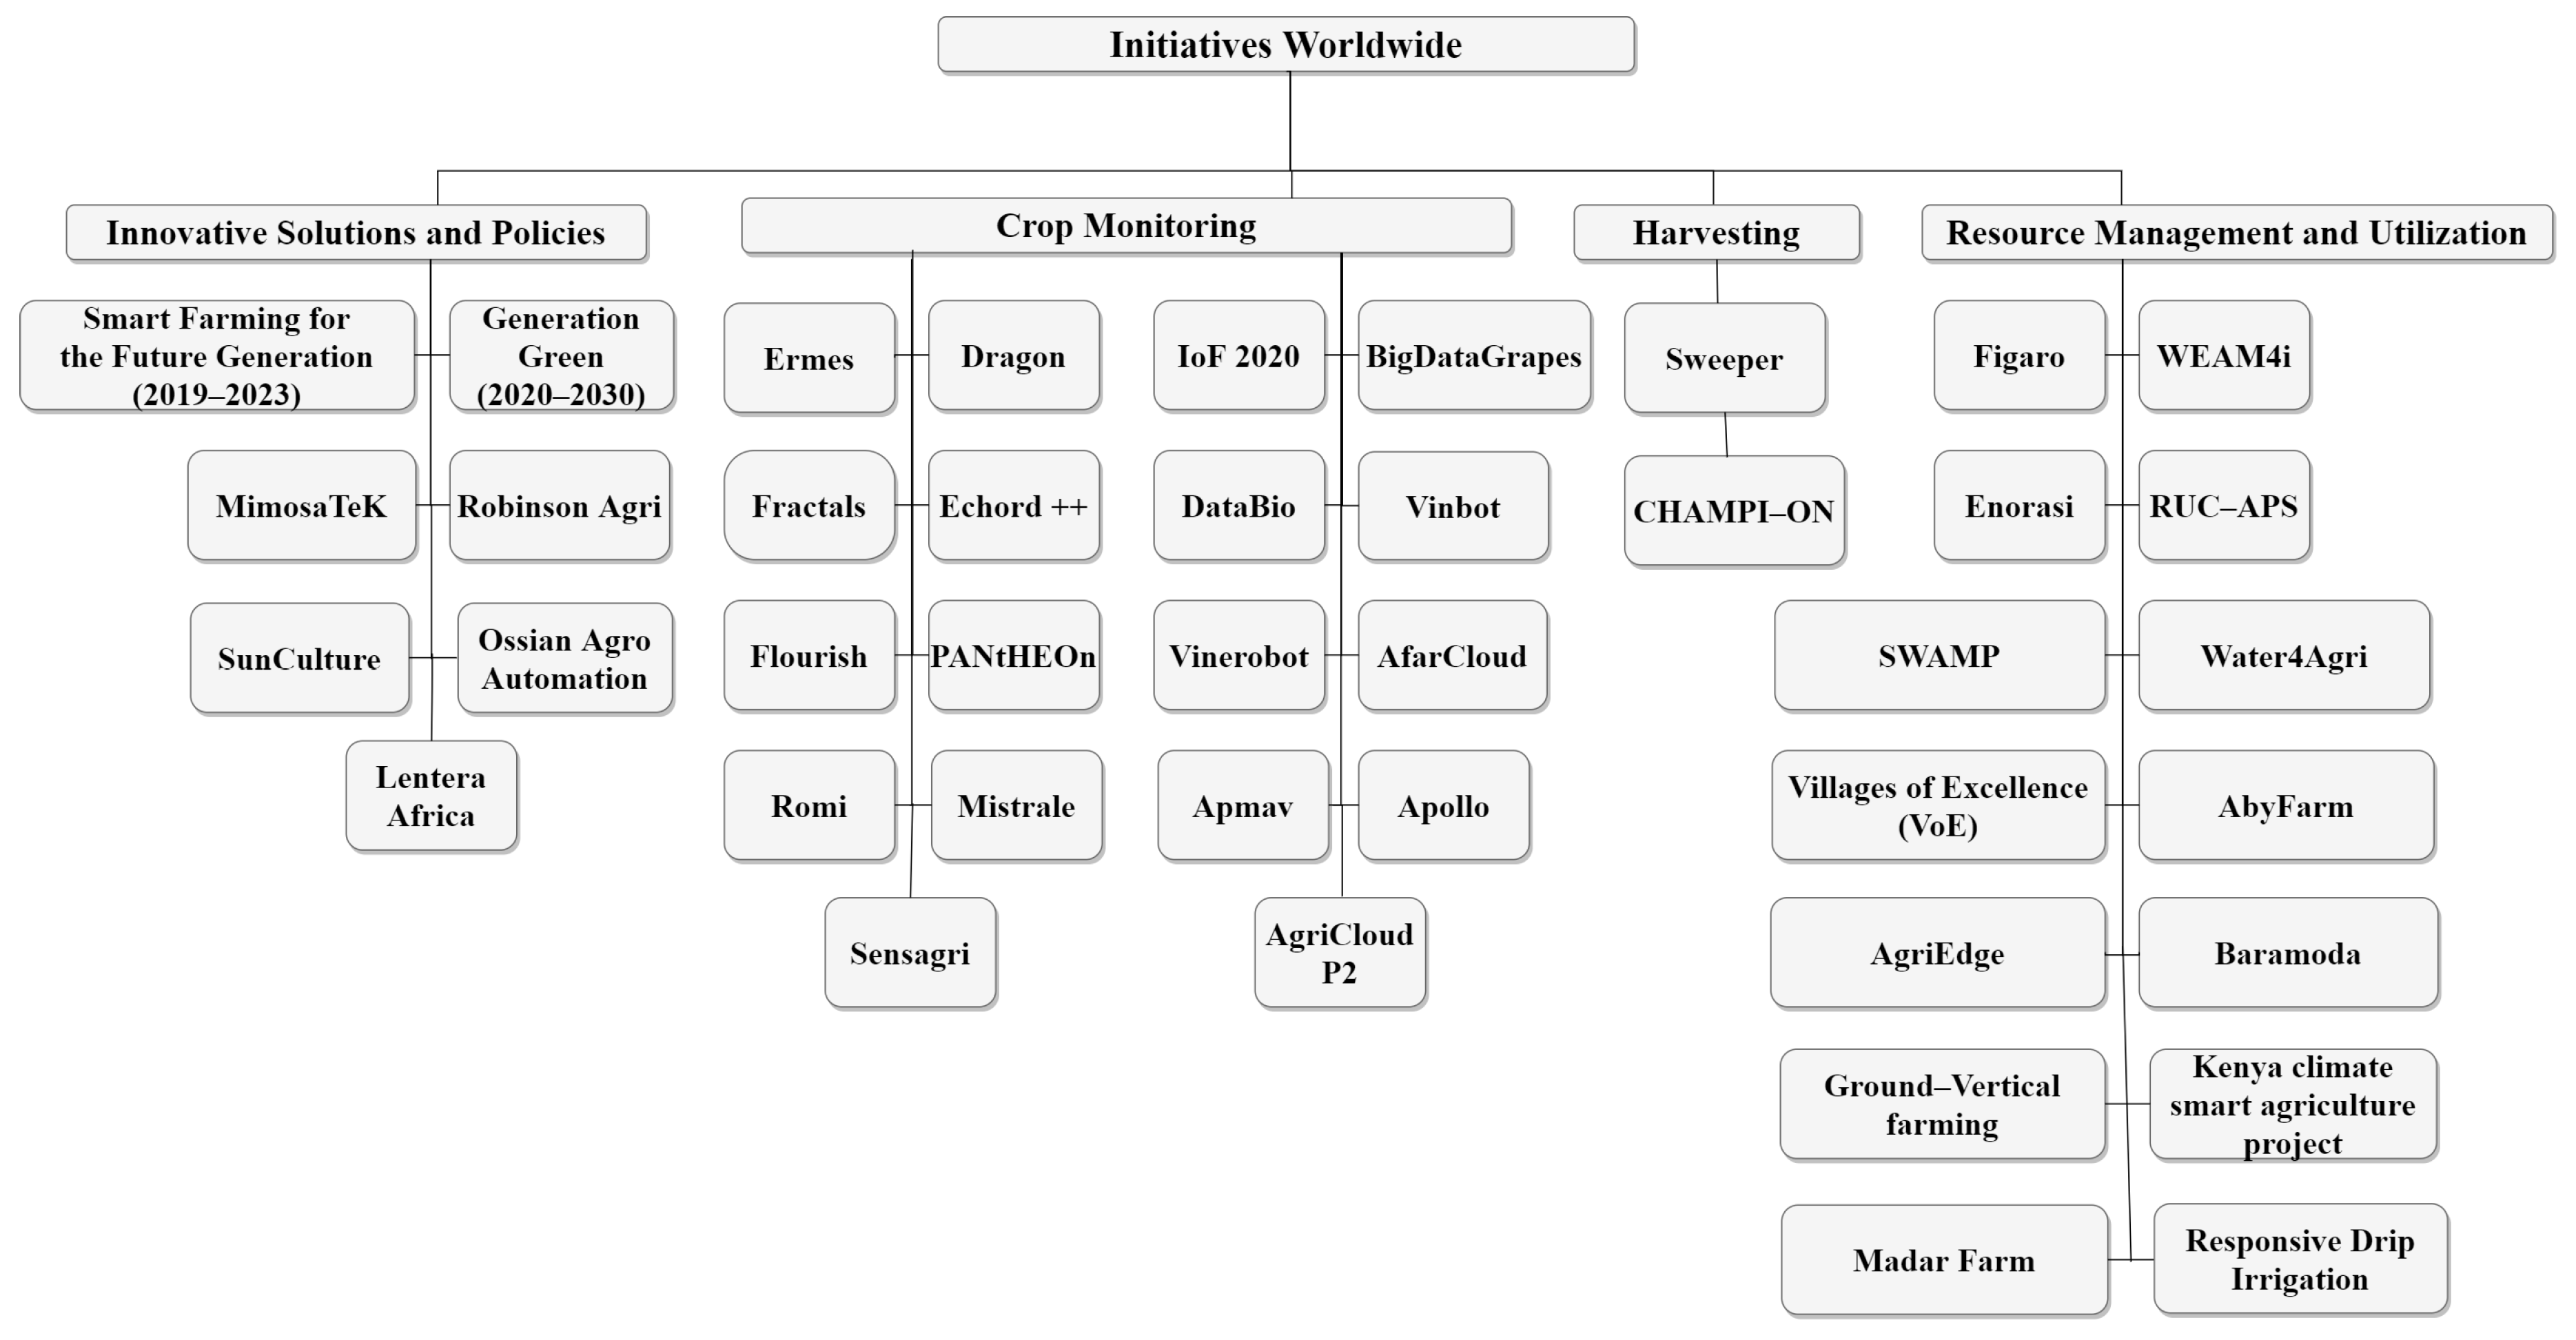
\includegraphics[width=\columnwidth]{agriengineering-04-00029-g005}
    \caption{A classification of active European Union funded project in the area of Digital Agriculture (from \cite{agriengineering4020029})}
    \label{fig:euprojects}
\end{figure}

In Europe, the European Community has funded many project that integrate ICT technologies and Digital Argriculture, we see in Figure \ref{fig:euprojects} from \cite{agriengineering4020029} a collection of active research project and startups, classified in different areas, such as:  \emph{Crop Monitoring}  (the largest one), \emph{Harvesting}, optimization of \emph{Resource Managements} and \emph{Innovative Policies and Solutions} with more than $41$ iniziatives. In Table \ref{fig:table-worldwide} another list of worldwide projects that are actually funded, with a increasing role for African and Middle-East countries.

In this paper, we present the activities of \textsc{TEBAKA}: a national project funded by PON-FESN (Europen Union Social Fund) dedicated to develop the adoption of Digital Agriculture in the south part of Italy (Mezzogiorno) and in particular in Apulia (Puglia). The project span four years, from 2020 to 2024 and with an overall budget of 8.5 Million Euro it put together more than 20 partners from industry, two university, several national research institutions of Italian CNR, and private partners with a mixed background (someone more oriented to ICT services, someone more related to agronomy). 
We discuss the project in the following section, but we want to summarize here the key ideas involved. The project goals is to develop a new generation of decision support system for agronomists for the culture of grain, vine and olive: for this goal, we conduct a large campaign of data acquisition, with measurements taken directly on the culture and soil, spanning two full year. Moreover, all measurements will be taken at the same time of satellite observation (with Sentinel 2), drone observations equipped with a multi-spectral camera and with aircraft. This four levels of observation are unique in all the projects presented in the previous discussion, they allow a \emph{pyramidal representation} at different spatial resolution of the phenomena observed, and in different time. On top of this raw observations, we develop data-driven models (mostly based on \emph{neural networks}) that extract features from images related with the specific conditions of the annual crop life cycle.

The rest of the paper is organized as follow: in \ref{sec:tebaka} we review the project structure and management organization, the partnership and roles, the research goals and actual status; in \ref{sec:activities} we present some interesting original results obtained, in two different areas: in \ref{subsec:webapp} we describe a web application and the related backend, to support agronomist in large field to collect samples from different gps locations with the aids of smartphones and/or tablets, this is also strictly related to a well know problem about the \emph{optimal deployment of a sensor network in a field}; in \ref{subsec:segmentation} we explain why in the overall pipeline of analysis it is important to properly do a \emph{semantic segmentation} of the plant crown (foliage) and present a semi-supervised approach to the problem; in \ref{sec:related} we collected some of the most relevant works that shape the area, and finally we drawn in \ref{sec:conclusion} the conclusions.

\begin{figure}
    \centering
    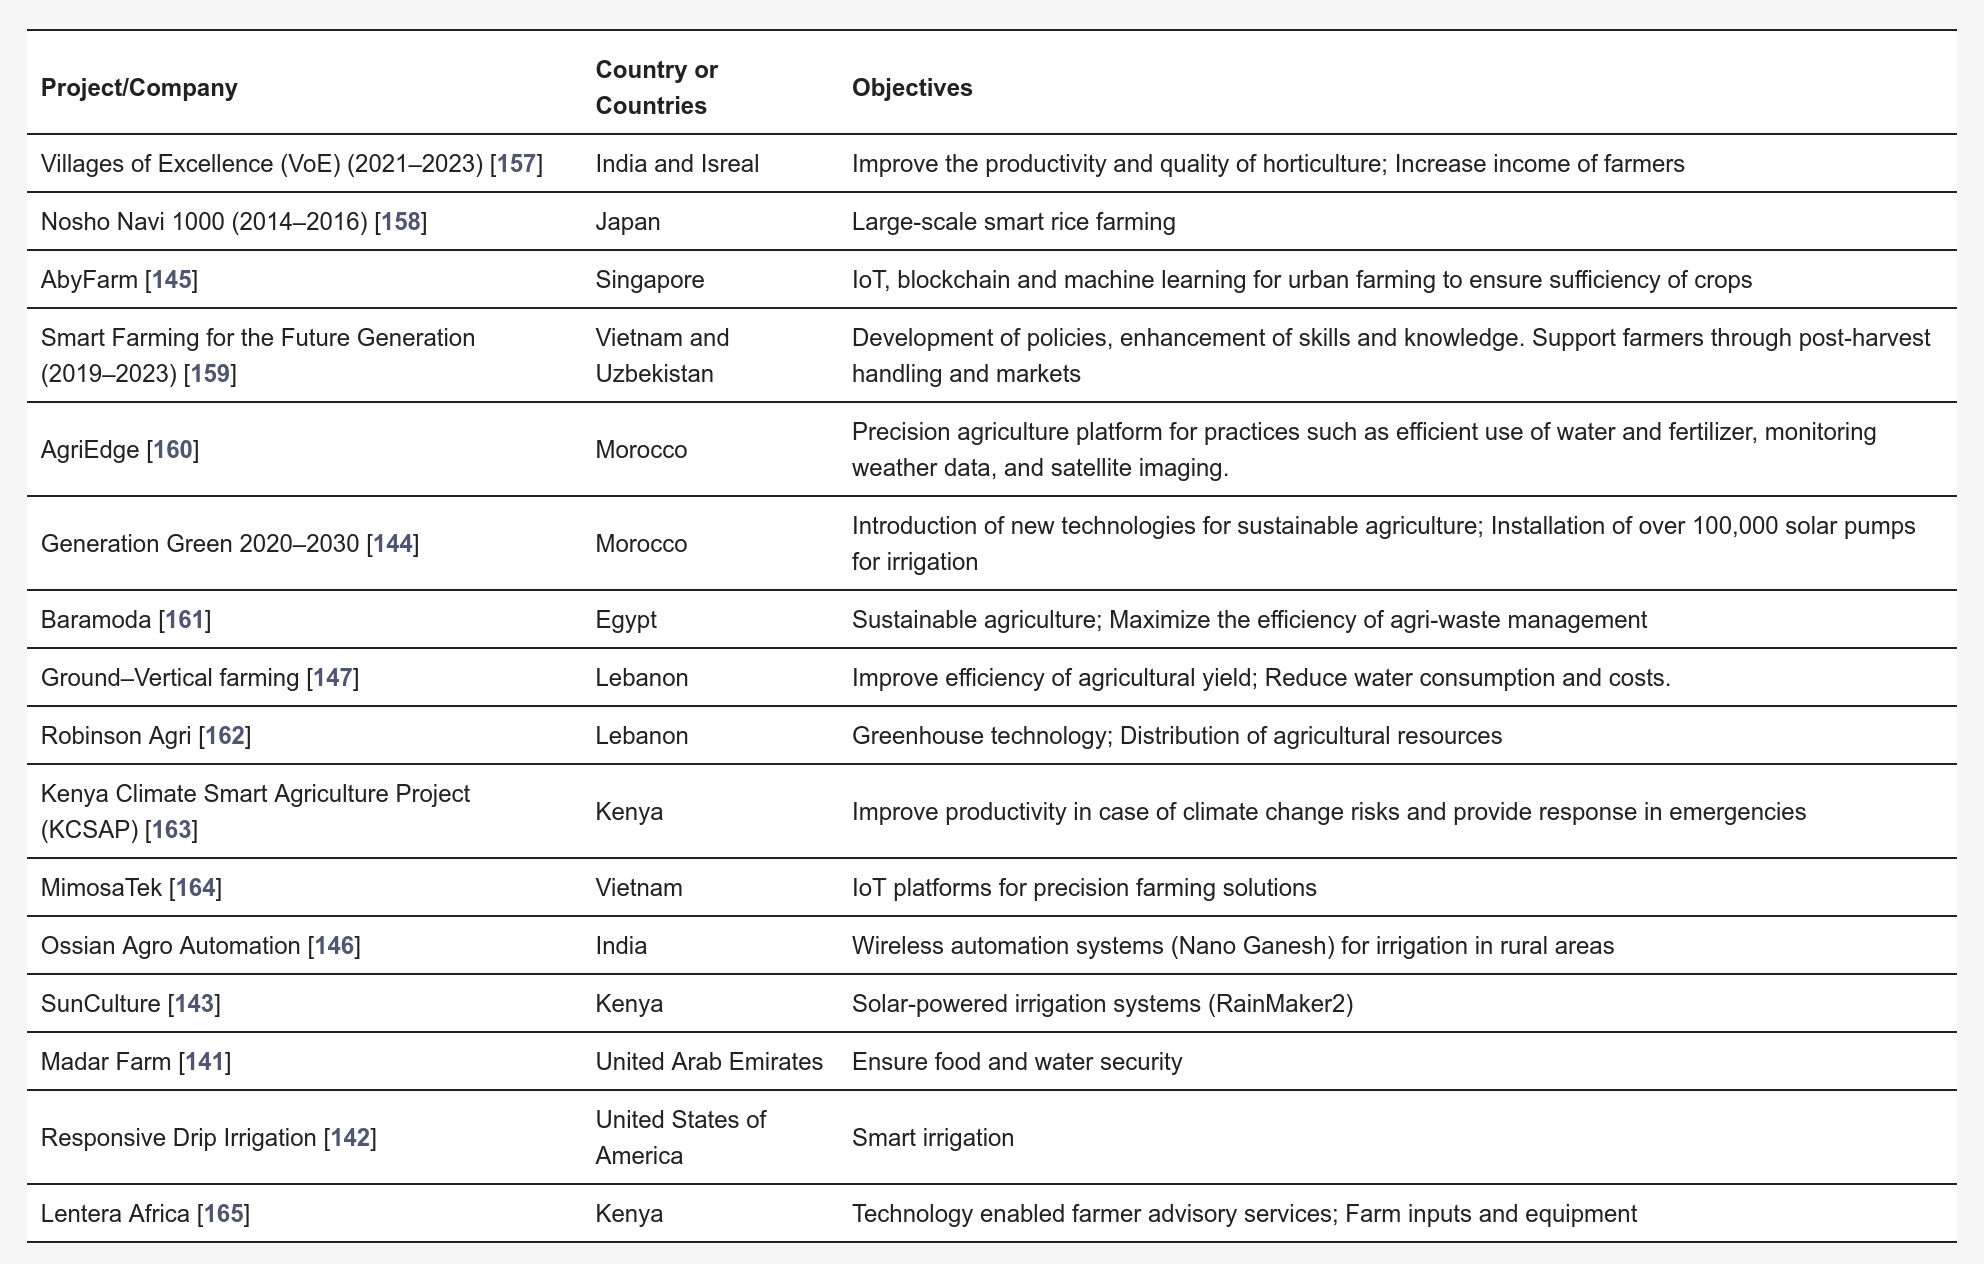
\includegraphics[width=\columnwidth]{research-table}
    \caption{A list of worldwide projects related to the area of Digital Agriculture (from \cite{agriengineering4020029})}
    \label{fig:table-worldwide}
\end{figure}

%--------- end of intro

\section{Tebaka Project Description}\label{sec:tebaka}

Tebaka is a “\emph{platform}” solution for crops of grain, vines and olive oil, all of which are significantly present in the sud of Italy, and will operate through stages of knowledge development and design / realization of prototype solutions that is articulated in four years (2020/2024) with the four major phases described in the following.

\textsc{Data Acquisition:}

\begin{itemize}
\item Analysis of the territory of Puglia, identification of the areas and parcels cultivated to observe, definition / authorization of the operational missions and their verification.
\item Definition of payload and cargo platforms of sensors to be used (on already operational satellites and on aircraft and land systems to integrate / develop), development of a control room for mission management and operational integration with a data acquisition and processing center.
\item Definition of data acquisition criteria from various platforms / pay loads during the various missions envisaged, verification of operational adequacy in the identified territories and basic processing of acquired data through representation in thematic maps.
\end{itemize}

\textsc{Analysis and Modelling Phase:}

\begin{itemize}
\item Definition of the theoretical models of the annual production cycles of the agricultural crops considered, of the fusion criteria of data from multisensor sources, of the criteria for the analysis of the data acquired in the missions, of the criteria for the realization of the data driven models with the use of artificial intelligence logic and deep learning, of criteria for their integration with theoretical models, and the implementation of integrated and validated basic models.
\item Development of Intensive Data Acquisition Activity from Payloads / Platforms for refinement of models, realized by means of large amounts of data processing, definition of criteria for identifying potential critical factors and development of models / support decision systems for their management, development of the design and the prototype of the complete system.
\end{itemize}

\textsc{Prototype Development:}

\begin{itemize}
\item Realization of the prototype of an integrated platform composed of technological systems (satellites, manned and unmanned aircrafts, manned and unmanned land vehicles and fixed stations, payloads of sensors with different characteristics and performance, storage environments of large amounts of data and applications in the field of artificial intelligence for data manipulation;
\item The building of data driven models; the development of models and relationships between the observed phenomena elements realized with machine learning logic, data analysis, decision support systems) in order to develop a product / service for the world of crops with different types of extension on the territory (horizontal for grain, vertical for vine and mixed for the olive tree, others with comparable characteristics) to be offered to various actors operating in the world of innovative agriculture such as Public Organizations, Category Associations, Service Providers, Agricultural Companies d medium / large national and international levels, possibly complementing the proposed solution with other complementary existing or developing ones.
\end{itemize}

The proposed project has as its ultimate goal the creation of an innovative product / service prototype for agriculture, in particular for grain, olive and vine crops, oriented to provide instruments and knowledge for the acquisition and to generate information for management decisions, in particular to provide guidance in the initial stages of potential and / or critical manifestations and to guide the best-performing actions. The concept of working with models of annual production cycles also allows to better estimate the final industrial result, and therefore economic, of the productions in progress.

The constitution of the advisory board presented is the basis for both orienting / validating the proposed solution and disseminating the product / service proposal to the agricultural world that is increasingly recognizing and utilizing intelligent agriculture solutions for the optimization of missions of the various actors involved. During the development of the project, a comparison will be made between the participants and external stakeholders to evaluate the possibility / opportunity to realize a spin-off that, through the acquisition of the platform, can to industrialize, maintain and use it as a basis for providing advice / services on the market.

It is primarily usefull for large territorial use but still maintains its validity for smaller areas, encouraging in this regard the concept of joint use among multiple actors in order to benefit from innovative solutions through affordable costs. The solution enables both private and public entities to design high value added services. For private sector it can be usefull for consultancy while for the public actors it can support policies and actions in order to favour the development of the agricultural production.

The articulation of activities, and hence the results that can be achieved for each one, also creates value in both the realization / improvement of system components (better bid ability in their business markets) and the development of internal knowledge and capabilities to be used also for development of other products / services / solutions. The greatest knowledge gained from the university and research entities can also offer better and consulting skills in the market, also contributing to the enhancement of the territory.

\section{Project Activities}\label{sec:activities}
% main part: flow of activities, from observation to 
% practical agronomic practice.

\subsection{An online Data Collection Application for Agronomist on the Field}\label{subsec:webapp}
% remote sensing platforms, big players, open satellite data.
% impact and use of them, spectral indexes, IoT, smart
% deployment. Web app for agronomy, for field data collection.

\lipsum[2-3] %<- to be filled

\subsection{Semi-Supervised Semantic Segmentation of Plant Crown}\label{subsec:segmentation}
% Image analysis using deep learning, role, goals result.

Segmentation is a recurrent task in literature regarding precision agriculture: the information provided by a pixel-wise classification map can by used to solve different domain specific tasks (\cite{s21051617,rs14061523,Egli20201}), e.g. biovolume estimation, tree crowns mapping, estimate the distribution of the popuilation for different species , monitoring changes in green areas. 
%\todo{list someone}
We introduce this task, in TEBAKA, in order to monitor the grow of
plants and in particular the \emph{volumetric leaf area} and its evolution across time.

The two main remote sensing technologies that have been used over the years are satellite and UAV imagery, each one having his pros and cons. Even if satellite imagery has also been used successfully by several authors\cite{ruswurm_multi-temporal_2018,daudt_fully_2018,ienco_land_2017},
the unmanned aerial vehicles (UAVs) have proven to be a game-changing technology for various reasons. The main one is that for the majority of agriculture challenges, there are strict resolution requirements that satellite imagery cannot satisfy. These requirements can be meet by UAV imagery while keeping costs acceptable. Satellite imagery is the best choice only if we have to deal with large scale observable phenomena\cite{gurumurthy_mango_2019,guirado_mask_2021}, since specific patterns can be observed only from a certain scale onward. For these reasons, we decided to choose UAV imagery as data source.

In agronomic, there are many well known indexes that are used to assign a score to each pixel. These indexes are often linear (or non-linear) combination of spectral channels, and have proven to be highly correlated to specific characteristics available in areas that have and index score above a certain threshold. The Normalized Difference Vegetation Index (NDVI) is an index, between $-1$ and $1$, that can be used to assess whether or not the target pixel contains live green vegetation.
%The Normalized Difference Water Index (NDWI) is another index used to estimate the leaf water content at canopy level.
Even if NDVI thresholding can be used to produce a segmentation map of a UAV image, there are many issues that make it a non-optimal choice. Different objects with the same spectrum obtains the same score, even if they belong to different classes. Moreover, NDVI does not consider local properties and patterns. Image analysis through deep learning has proven to provide state of the art solutions for instance/semantic segmentation in different domains. For this reason, this method has been widely used in precision agriculture in the last decade.

However, supervised deep learning methods require large, hand-labelled datasets, that are carefully prepared by domain experts, in fact, in all the works examined, and reviewed in the next section, the labelling is carried out by agronomists. In our work, we propose an original solution for the automatic labeling of UAV images containing vineyards and olive trees. We tested this method, by using this data-set to train a well-known semantic-segmentation neural network model, the entire system can be considered a self-supervised model, with the advantage that the self-labelling pipeline, can be used to label any plant species without the costly manual labour of a domain expert (in this case an agronomist). To the best of our knowledge, there is no other work using a similar solution in this domain, in particular we are not aware of a single method that can be used on more a single culture type. 

The self supervised pipeline is a system that takes as input an hyper-spectral orthomosaic and returns the set $\mathcal{D}$: \[
\mathcal{D} = \{\, (x_i,y_i):i \in \{1...N\}\,\}
\] where $x_i$ represents the $i$-th tile of the input orthomosaic, $y_i$ is the ground truth mask for $x_i$ and $N$ is the total number of collected tiles i.e. the size of the dataset.
% \todo{explain what is $i$, i.e. the size of the dataset, introduce a variable (maybe, 'we consider N the size of the dataset and $i$ range over N}. OK
Masks and tiles have the same spatial resolution, but masks have only one channel, i.e. they are bitmaps, with the value of each pixel be equal to 0 (background) or 255 (vegetation) (we still use 8 bit for each pixel). This representation is useful for visualisation purposes. During the development of the machine learning model, we represented 0 and 255 with the one-hot-encoding.
%\todo{it is a detail, or it is important?}

Only two classes have been assigned to speed up prototyping, but their number can be easily extended, i.e. by labelling each species with a different value. The self supervised pipeline (Figure \ref{fig:entirepipeline}) works as follow:

\begin{itemize}
    \item The NDVI is computed pixel-wise from the multispectral input orthomosaic and stored as a single-channel image. The NDVI formula is:
    \[
    NDVI = \frac{NIR-R}{NIR+R}
    \]
    Where $NIR$ (Near Infra Red) and $R$ (Red) bands are respectively stored in the 6th and the 10th channels of our source orthomosaic.
    \todo{L: aggiungere descrizione NIR e motivo formula NDVI}
    %\todo{explain NIR, they don't know about it, and the general idea of why ndvi is computed in that way..find everything on wikipedia, just one more phrase}
    \item The NDVI map is the input to a Tunable Denoising Module that is part of the semi-supervised model. This component (shown in Figure \ref{fig:tunable_module}) is a stack of different well known image processing techniques executed sequentially. 
    The module is executed by fixing a set of parameters that govern its operation. In our experiments, the values of these parameters were found by drawing inspiration from the search criteria for hyperparameters used in machine learning (e.g. grid search inside intervals considered reasonable).
    This module produces the pixel-wise ground truth map for the entire hyperspectral source orthomosaic. The tunable parameters of this module are 5 (highlighted in red in previous image). Values $th_1$ and $th_2$ governs the two tresholding stages, while $sw$, $tw$ and $str$ respectively represents the search window size, the template window size and the strength of the fast non local means denoising method. For the dilation and the erosion, we used kernels containing only 1 with size $3\times3$ and $5\times5$.
    An erosion follower by a dilation is called opening. The opening is a smoothing filter and the specific behavior depends on the kernel size and content. An opening preserve as much as possible regions having similar structure respect to the kernel, while removing those different. Our kernels with all 1's allow to remove isolated groups of pixels, while their dimension governs the minimum size that groups of pixels must have in order to be preserved. Kernel size and content could be governed introducing some parameters, although in our experiments we achieved good results with static kernels.
In our case, they serve to remove groups of isolated pixels classified as plants 
    %\todo{maybe write a single phrase on the high level task of this? like 'removing debris or small components in the image??}
    \item The orthomosaic/ground truth are both split in many tiles of a fixed size. We pairwise store each input tile and its corresponding ground truth tile. The size of the tiles was chosen consistently with the size of the input expected from the semantic segmentation deep learning model we trained.
\end{itemize}

Before storage, pairs of tiles containing insufficient information are discarded. Specifically, if the pixels in the truth map describing vegetation are fewer than a given threshold, then the pair is discarded. In our experiments, we labeled $906$ tiles (net of rejected ones) starting from $5$ UAV orthomosaics acquired in $2$ different areas of interest \todo{and spanning an area of ..km$^2$}.

Flights for the acquisition were performed in a temporal window spacing from the $26$ May $2022$ to $30$ Sep $2022$. The semantic segmentation model we chose for training is the U-Net 
\cite{ronneberger_u-net_2015}, with some modifications, 
%\todo{it is not up to you to write 'trivial' for tour job, you are selling something..so nothing is trivial}
for example making it capable of handling the 10 channels for the images in input. 

%In addition, we used a matrix full of 1's as the loss regularisation matrix, thus making it irrelevant. 

We chose U-Net over other similar architectures for several reasons: it has fewer parameters than competing networks. Moreover, it was originally proposed to solve a task of similar complexity (biomedical image segmentation) with excellent results, which were then replicated on use cases very similar to ours. Lastly, in these publications (and also in the original work) the U-Net was trained from scratch with datasets of comparable size to ours (often even smaller).
%\todo{if you don't need to reference the (a)(b)(c), why don't just write the paragraphs, without them??}

We performed several training runs in order to cross validate different hyperparameters: decay rate, learning rate, number of epochs, and batch size. \todo{ok, and we are happy ;), so ....discuss the result of the training in fig 5.}

\todo{ok, well written, not bad, continue, put also something in the related work.}

\begin{figure}
    \centering
    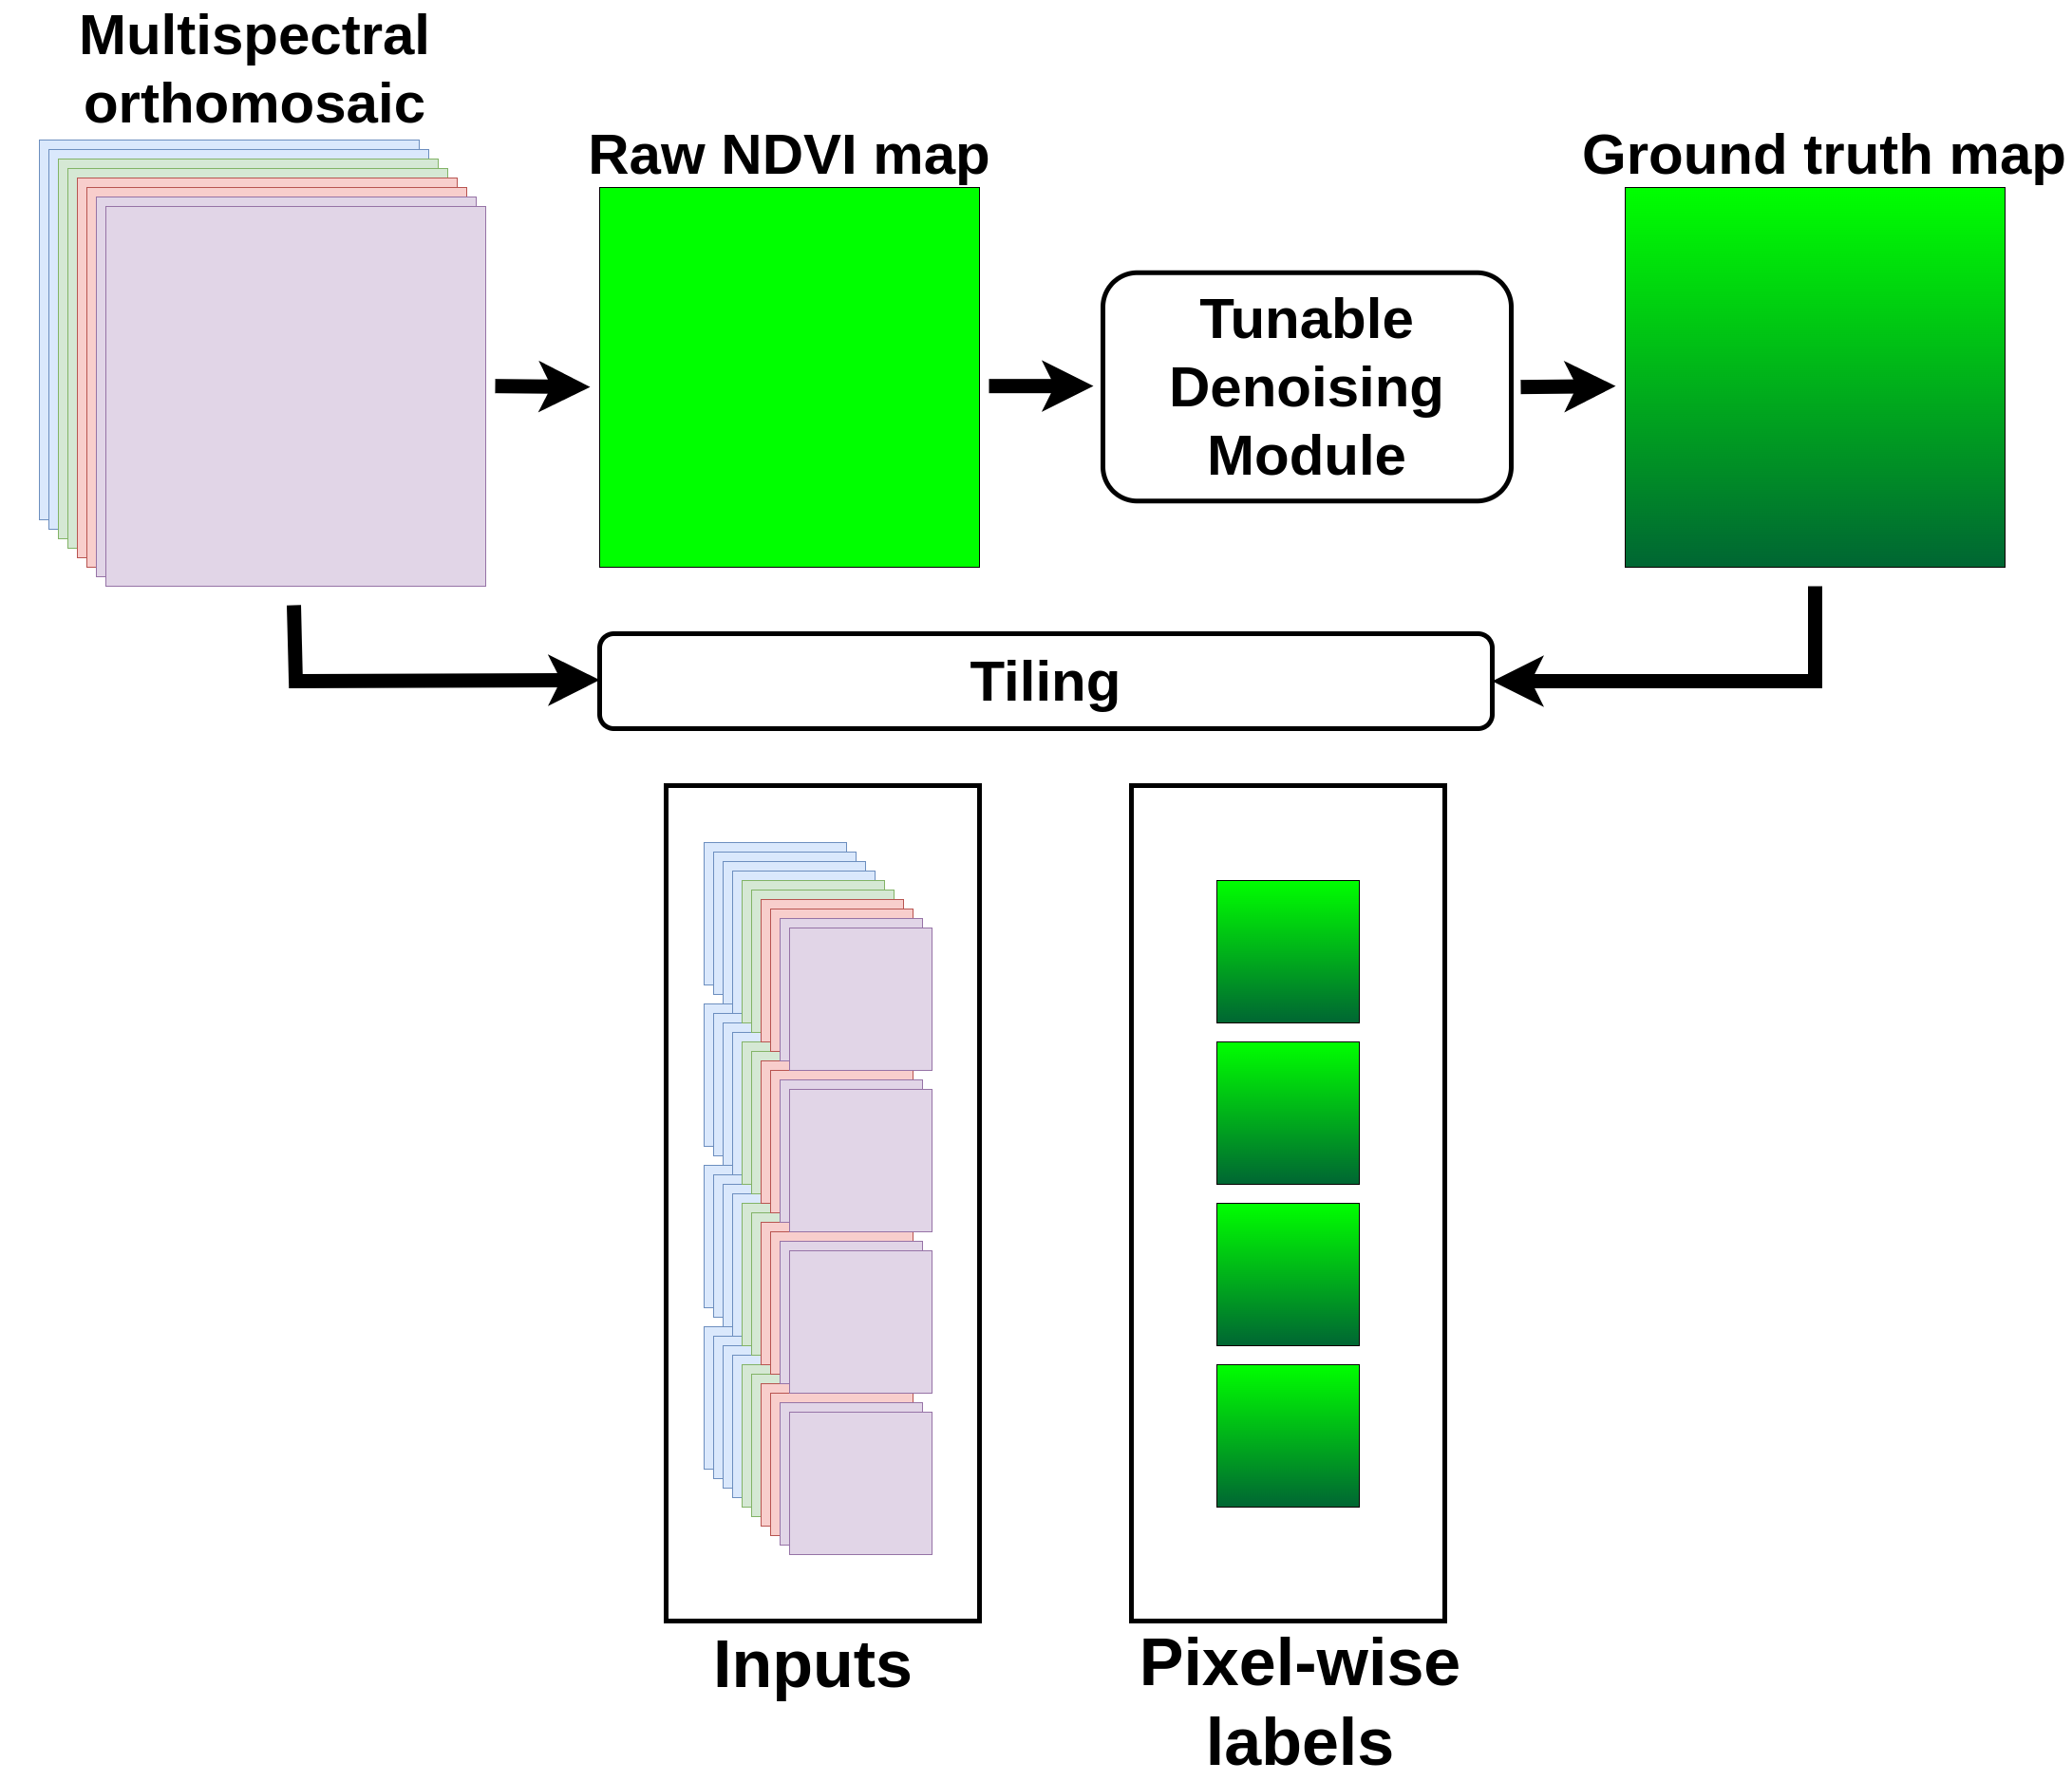
\includegraphics[width=\columnwidth]{pipeline1}
    \caption{Graphical representation of the entire self-supervised pipeline.}
    \label{fig:entirepipeline}
\end{figure}

\begin{figure}
    \centering
    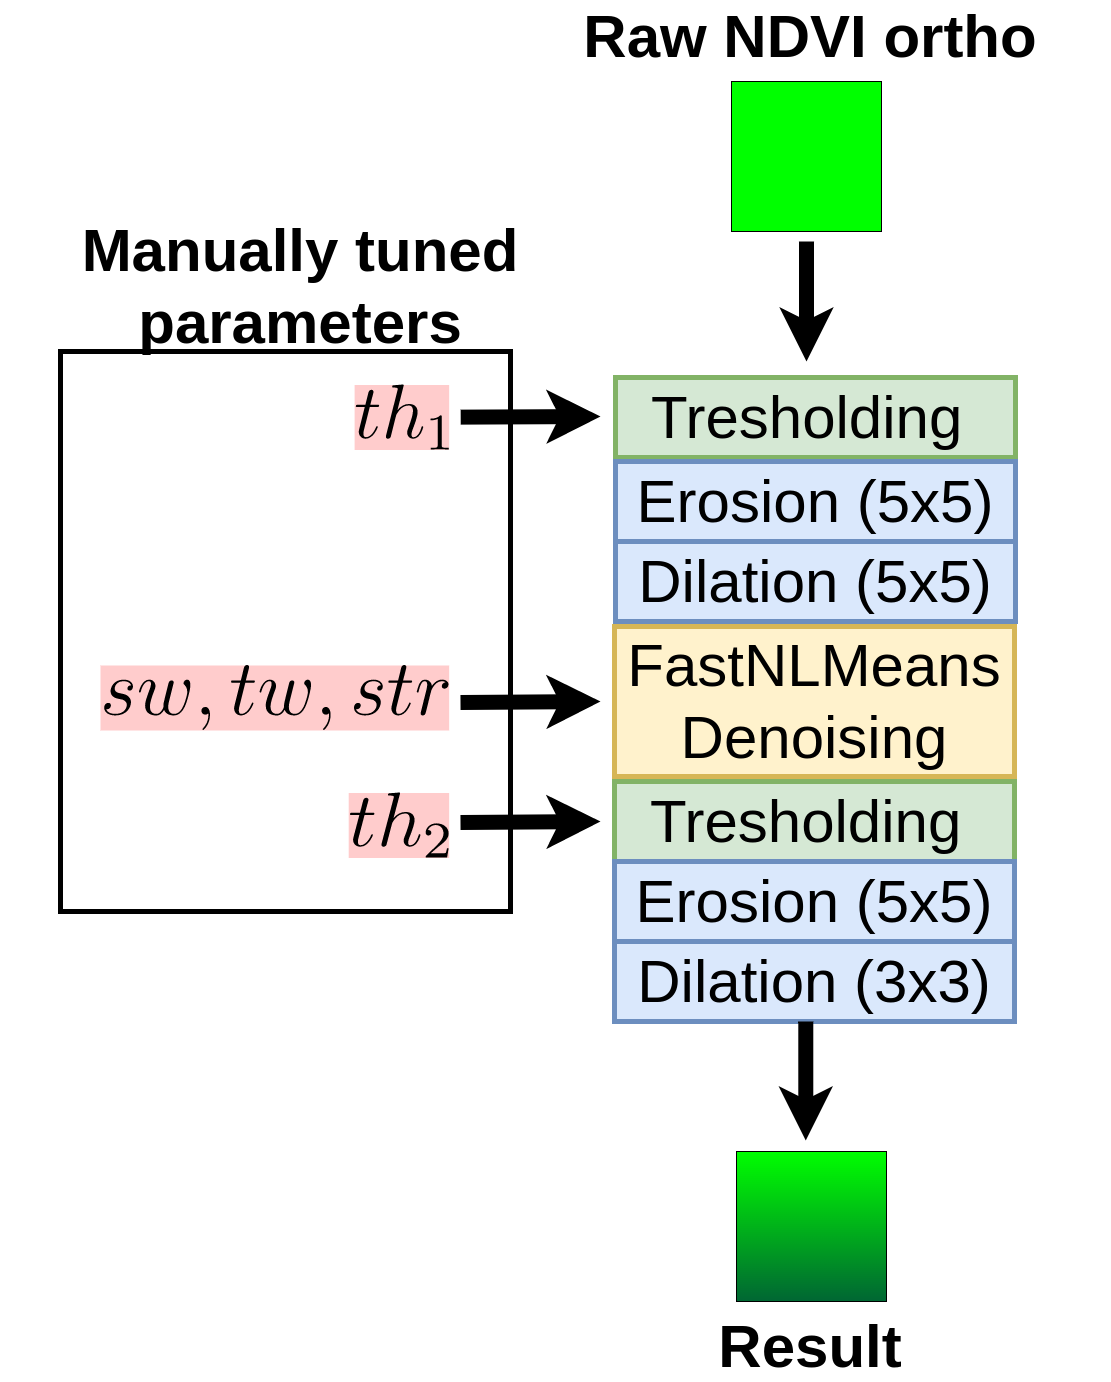
\includegraphics[width=0.8\columnwidth]{tunable_module}
    \caption{Schema of the Tunable Denoising Module.}
    \label{fig:tunable_module}
\end{figure}

\begin{figure}{\centering%
%
      \begin{subfigure}[b]{0.45\columnwidth}
         \centering
         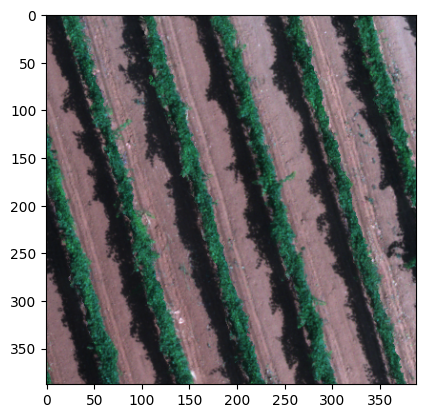
\includegraphics[width=\columnwidth]{vite}
         \caption{}
         \label{maskplot:a}
     \end{subfigure}%
%
     \begin{subfigure}[b]{0.45\columnwidth}
         \centering
         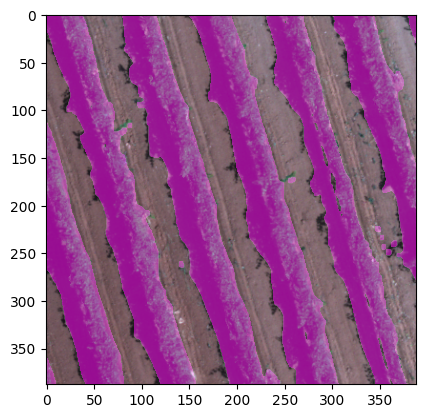
\includegraphics[width=\columnwidth]{vite_GT}
         \caption{}
         \label{maskplot:c}
     \end{subfigure}}\\%
%       
     \begin{subfigure}[b]{0.45\columnwidth}
         \centering
         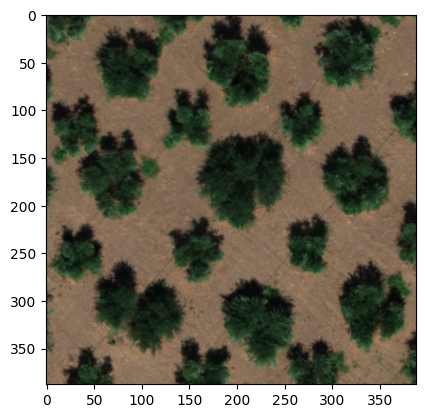
\includegraphics[width=\columnwidth]{ulivo}
         \caption{}
         \label{maskplot:input_tile2}
     \end{subfigure}%
%
     \begin{subfigure}[b]{0.45\columnwidth}
         \centering
         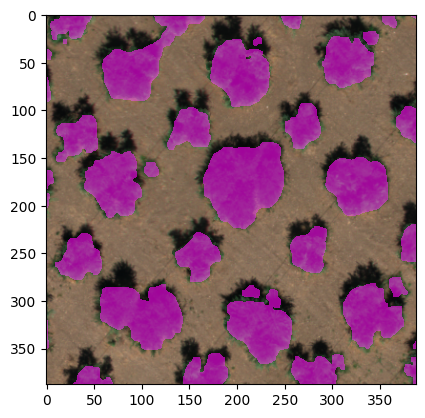
\includegraphics[width=\columnwidth]{ulivo_GT}
         \caption{}
         \label{maskplot:patch_inf2}
     \end{subfigure}%
%        
     \caption{(a) Input tile, vineyard; (b) Overlay between the previous input tile and the result produced by our self supervised pipeline; 
     %(c) Overlay between the vineyard input tile and his ground truth mask. 
     (c),(d) are the same but for olive trees}
     % don't break lines manually NEVER
\end{figure}

\begin{figure}{\centering%
%
      \begin{subfigure}[b]{0.3\columnwidth}
         \centering
         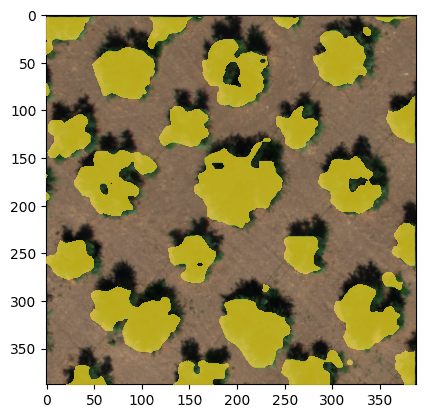
\includegraphics[width=\columnwidth]{ULIVO0INF}
         \caption{}
     \end{subfigure}%
%
     \begin{subfigure}[b]{0.3\columnwidth}
         \centering
         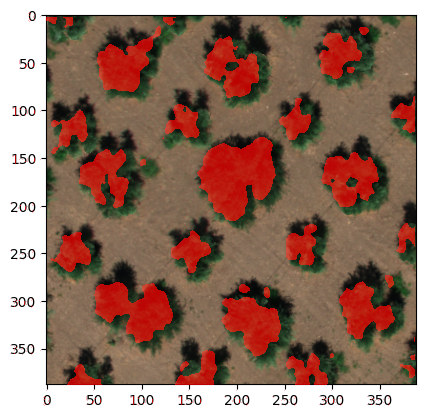
\includegraphics[width=\columnwidth]{ULIVO1INF}
         \caption{}
     \end{subfigure}}%
%       
     \begin{subfigure}[b]{0.3\columnwidth}
         \centering
         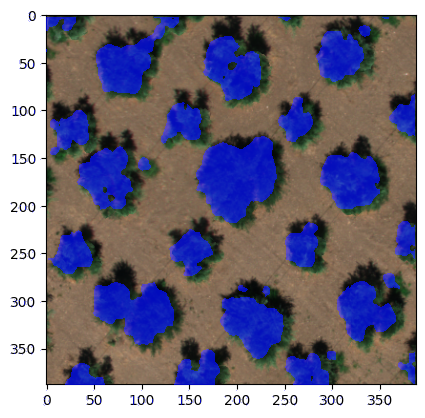
\includegraphics[width=\columnwidth]{ULIVO2INF}
         \caption{}
     \end{subfigure}%
% 

      \begin{subfigure}[b]{0.3\columnwidth}
         \centering
         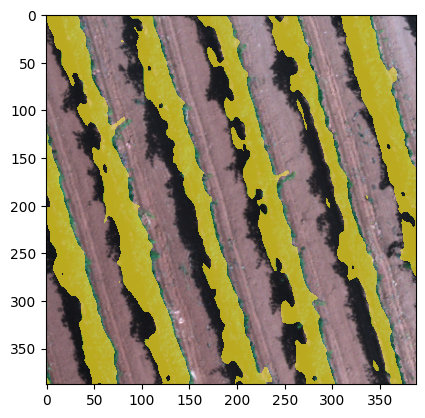
\includegraphics[width=\columnwidth]{VITE0INF}
         \caption{}
     \end{subfigure}%
%
     \begin{subfigure}[b]{0.3\columnwidth}
         \centering
         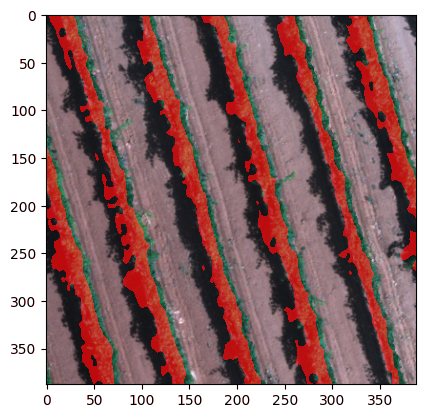
\includegraphics[width=\columnwidth]{VITE1INF}
         \caption{}
     \end{subfigure}%
%       
     \begin{subfigure}[b]{0.3\columnwidth}
         \centering
         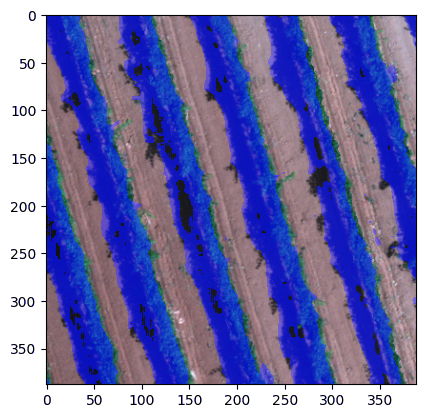
\includegraphics[width=\columnwidth]{VITE2INF}
         \caption{}
     \end{subfigure}%
% 

     \caption{Overlay between the input tiles and the result pro}
     % don't break lines manually NEVER
\end{figure}


\section{Related Works}\label{sec:related}
% a panoramic view of the best literature, focus on technology.

In \nocite{*} we have...\todo{contribute here}


\section{Conclusion}\label{sec:conclusion}

In this paper we presented the TEBAKA project, and discuss its relevance in the overall scenario of national or international project related to Precision Agriculture. We emphasized the originality of the project, in particular how it lives at the intersection of communications problems related to satellite data management and IoT deployment on the field, and computational problems, i.e. new advanced data-driven ML models that better integrate all knowledge of the domain.
We presented a case of a particular task, \emph{image semantic segmentation} of the crown of olive trees or rows of grape plants and shown how to implement an original semi-supervised network that produce the segmentation with unexpected accuracy. In the next year of the project we will obtain new data from the second phase of data acquision on the filed, to validate the models and improve their correspondace with data measured directly from the culture. There is still a large gap between the research and goals of TEBAKA and the actual industrial adoption of precision agriculture from real actors of the industry, and we will work on disseminating the project result in order to inprove this scenario.


\section*{Acknowledgment} Put sponsor 
acknowledgments in the unnumbered footnote on the first page.

\printbibliography

\end{document}
